% !TeX spellcheck = de_CH

% ========================================
% Thesis template by Michael Wieland
% Template version: v1.0
% ========================================

	
% Document
% ====================
\documentclass[11pt, a4paper, oneside, titlepage]{memoir}

% Package Imports
% ====================
% Packages
%% ========

%% Language and encodings
\usepackage[T1]{fontenc}
\usepackage[utf8]{inputenc} % Due to vowels.
\usepackage[ngerman]{babel} % Choose english, american, ngerman
\addto{\captionsngerman}{\renewcommand{\abstractname}{Abstract}}
\usepackage{datetime} % time depending on locale

%% Layout
\usepackage{multicol}
\usepackage{lscape}
\usepackage{pdflscape}
\usepackage{float}
\usepackage{fancyhdr} %To customize the headers and footers.

%% Font
\usepackage{pifont}
\usepackage[sc]{mathpazo}
\usepackage[german=swiss]{csquotes} % swiss quotes with \enquote{Text}

%% Math
\usepackage{amsmath,amsfonts,amssymb,mathrsfs, mathtools}
\usepackage[amsmath,thmmarks]{ntheorem}

%% Graphics, figures, listings
\usepackage{graphicx}
\usepackage[table]{xcolor}
\usepackage{caption}
\usepackage{subcaption}
\usepackage{wrapfig}
\graphicspath{ {images/} }
\usepackage{tcolorbox}

%% Tables
\usepackage{array}
\usepackage{ltxtable}
\usepackage{tabularx}
\usepackage{tabulary}
\usepackage{multirow} % Multi-rowed cells in tabulars
\usepackage{booktabs} % \cmidrule or \addlinespace
\usepackage{rotating} % rotate table
\usepackage{longtable}
\usepackage{dcolumn}
\renewcommand{\arraystretch}{1.25}

%% Include external pdf
\usepackage{pdfpages}

%% References
\usepackage{varioref} % TODO add example refs

%% Bibliography
\usepackage[style=numeric,sorting=ynt,backend=biber]{biblatex}
\addbibresource{references.bib}

%% Glossary
\usepackage{xparse}
%\usepackage[hidelinks]{hyperref}
\usepackage[nomain,acronym,toc]{glossaries}

\DeclareDocumentCommand{\newdualentry}{ O{} O{} m m m m } {%
	\newglossaryentry{gls-#3}{name={#5},text={#5\glsadd{#3}},
		description={#6},#1
	}%
	\newacronym[see={gls-#3},description={#5},#2]{#3}{#4}{#5\glsadd{gls-#3}}%
}

\glsenablehyper
\makeglossaries

\loadglsentries{glossar-terms}



%% Code listings
\usepackage{listings}

\definecolor{DarkPurple}{rgb}{0.4,0.1,0.4}
\definecolor{DarkCyan}{rgb}{0.0,0.5,0.4}
\definecolor{LightLime}{rgb}{0.3,0.5,0.4}
\definecolor{Blue}{rgb}{0.0,0.0,1.0}
\lstdefinestyle{eclipse-style}{
	language=Java,  
	columns=flexible,
	showstringspaces=false,     
	basicstyle=\footnotesize\ttfamily, 
	keywordstyle=\bfseries\color{DarkPurple},
	commentstyle=\color{LightLime},
	stringstyle=\color{Blue}, 
	escapeinside={(*@}{@*)}, % latex scope within code      
	breaklines=true,
	breakatwhitespace=true,
	showspaces=false,
	showtabs=false,
	tabsize=4,
	morekeywords={length},
	numbers=none,
	frame=single,
}
\lstset{style=eclipse-style}

\usepackage{adjustbox} %for step-by-step instructions

% to draw folder structures
\usepackage{dirtree}

% to draw
\usepackage{tikz}

% to show keyboard keys
% usage: \menu{File, Save As...}
% usage: \directory{adv-ui/ui-core}
% usage: \keys{\cmd+\shift+S}
\usepackage{menukeys}

% Hyperlinks
% Must be loaded at the end!
\colorlet{purple}[rgb]{red!75!green!50!blue}
\usepackage[colorlinks=true,linkcolor=purple,citecolor=purple,filecolor=black,anchorcolor=black, urlcolor=black, runcolor=black, menucolor=black]{hyperref}

% Document Information
% ====================
\newcommand\thesisAuthorA{Author A}
\newcommand\thesisAuthorB{Author B}
\newcommand\thesisTitle{Titel}
\newcommand\thesisSubject{Bachelorarbeit}
\newcommand\thesisUniversity{Hochschule für Technik Rapperswil}
\newcommand\thesisDepartment{Abteilung für Informatik}
\newcommand\thesisAdvisor{Betreuer}
\newcommand\thesisExpert{Experte}
\newcommand\thesisCounterreader{Gegenleser}
\newcommand\thesisKeywords{java, hsr}
\newcommand\thesisPeriod{Zeitraum: 19.02.2018 - 15.06.2018}
\newcommand\footerTitle{ABC}

\hypersetup{
	pdfauthor={\thesisAuthorA, \thesisAuthorB},
	pdftitle={\thesisTitle},
	pdfsubject={\thesisSubject},
	pdfkeywords={\thesisKeywords}
}

% Settings
% ====================
%% Custom commands
%% Usage: \begin{my-theorem}
%% ===============
\newtheorem{theorem}{Theorem}[chapter]
\newtheorem{definition}[theorem]{Definition}

%% Box theorems commands
%% Usage: \begin{my-theorem}{title}{label}
%% ===============
\tcbuselibrary{theorems}
\newtcbtheorem[number within=section]{hint}{Hinweis}{fonttitle=\bfseries}{hnt}

\newtcbtheorem[number within=section]{warn}{Achtung}{colback=red!5!white,colframe=red!75!black}{}


%% Custom commands
%% ===============

\newcommand{\BigO}{\mathcal{O}}
\newcommand{\cmark}{\ding{51}}
\newcommand{\xmark}{\ding{55}}%%

%userstory counter
\newcounter{UserStoryCounter}
\newcommand{\userStory}{\setrow{\bfseries} \stepcounter{UserStoryCounter}
	US \arabic{UserStoryCounter}: }

%bold rows in table
\newcommand\setrow[1]{\gdef\rowmac{#1}#1\ignorespaces}
\newcommand\clearrow{\global\let\rowmac\relax}
\clearrow

%show priorities
\newcommand{\prio}[1][3]{%
	\setlength{\unitlength}{1ex}%
	\begin{picture}(1,1.8)
	\linethickness{0.3ex}%
	\textcolor{gray!15}{\multiput(0, 0.15)(0, 0.6){3}{\line(1,0){1}}}
	\multiput(0, 0.15)(0, 0.6){#1}{\line(1,0){1}}
	\end{picture}%
}

%New command for step-by-step instructions
\newenvironment{explanation}[2][]
{\begin{flushleft}
		\adjustbox{center=7cm,valign=c}{\includegraphics[width=6cm,#1]{#2}}%
		\begin{minipage}[c]{\dimexpr\textwidth-7cm\relax}}
		{\end{minipage}\end{flushleft}}
	
	
% new column Z with vertical and horizontal alignment = center and automatic width
\newcolumntype{Z}[0]{>{\centering\let\newline\\\arraybackslash\hspace{0pt}}X}%
\renewcommand\tabularxcolumn[1]{m{#1}}

% circles with numbers to reference images
% usage:  \circled{1}
\newcommand*\circled[1]{\tikz[baseline=(char.base)]{
		\node[shape=circle,draw,inner sep=2pt] (char) {#1};}}

\NewDocumentCommand \dotbox {o O{.5\linewidth} m O{3ex} O{\linewidth}}
{
	\begin{minipage}{7cm}
		\makebox[5cm][l]{\,.\dotfill}
		\\
		\makebox[5cm][l]{\,#3}
	\end{minipage}
}


\definecolor{redlight}{HTML}{EF9A9A}
\definecolor{red}{HTML}{D32F2F}
\definecolor{reddark}{HTML}{B71C1C}
\definecolor{purplelight}{HTML}{CE93D8}
\definecolor{purple}{HTML}{7B1FA2}
\definecolor{purpledark}{HTML}{4A148C}
\definecolor{bluelight}{HTML}{81D4FA}
\definecolor{blue}{HTML}{0288D1}
\definecolor{bluedark}{HTML}{01579B}
\definecolor{greenlight}{HTML}{A5D6A7}
\definecolor{green}{HTML}{388E3C}
\definecolor{greendark}{HTML}{1B5E20}
\definecolor{yellowlight}{HTML}{FFF59D}
\definecolor{yellow}{HTML}{FFFF00}
\definecolor{yellowdark}{HTML}{FFD600}
\definecolor{orangelight}{HTML}{FFCC80}
\definecolor{orange}{HTML}{F57C00}
\definecolor{orangedark}{HTML}{E65100}
\definecolor{brownlight}{HTML}{BCAAA4}
\definecolor{brown}{HTML}{5D4037}
\definecolor{browndark}{HTML}{3E2723}
\definecolor{graylight}{HTML}{EEEEEE}
\definecolor{gray}{HTML}{616161}
\definecolor{graydark}{HTML}{212121}
\definecolor{themegray}{HTML}{CED8E0}
% Document
% ====================

% Turn extra space before chapter headings off.
\setlength{\beforechapskip}{0pt}

\nonzeroparskip
\parindent=0pt
\defaultlists

% Chapter style redefinition
\makeatletter

%% Head and foot
\if@twoside
	\pagestyle{Ruled}
	\copypagestyle{chapter}{Ruled}
\else
	\pagestyle{ruled}
	\copypagestyle{chapter}{ruled}
\fi
\makeoddhead{chapter}{}{}{}
\makeevenhead{chapter}{}{}{}
\makeheadrule{chapter}{\textwidth}{0pt}
\copypagestyle{abstract}{empty}


% customize header and footer for chapter pages
\fancypagestyle{plain}{
	\fancyfoot[L]{\footerTitle}
	\fancyfoot[C]{}
	\fancyfoot[R]{\thepage}
}

%Customize headers and footers for normal pages
\pagestyle{fancy}
\fancyhead[LC]{}
\fancyhead[R]{\rightmark}
\fancyfoot[L]{\footerTitle}
\fancyfoot[C]{}
\fancyfoot[R]{\thepage}

%% Chapter style
\makechapterstyle{bianchimod}{%
	\chapterstyle{default}
	\renewcommand*{\chapnamefont}{\normalfont\Large\sffamily}
	\renewcommand*{\chapnumfont}{\normalfont\Large\sffamily}
	\renewcommand*{\printchaptername}{%
		\chapnamefont\centering\@chapapp}
	\renewcommand*{\printchapternum}{\chapnumfont {\thechapter}}
	\renewcommand*{\chaptitlefont}{\normalfont\huge\sffamily}
	\renewcommand*{\printchaptertitle}[1]{%
		\hrule\vskip\onelineskip \centering \chaptitlefont\textbf{\vphantom{gyM}##1}\par}
	\renewcommand*{\afterchaptertitle}{\vskip\onelineskip \hrule\vskip
		\afterchapskip}
	\renewcommand*{\printchapternonum}{%
		\vphantom{\chapnumfont {9}}\afterchapternum}}

\chapterstyle{bianchimod}

\copypagestyle{chapter}{plain}
\makeoddfoot{chapter}
{ADV}% Left
{}% Centre
{\thepage}% Right


% Set section and TOC numbering depth to subsection
\setsecnumdepth{subsection}
\settocdepth{subsection}

% Set captions to a more separated style for clearness
\captionnamefont{\sffamily\bfseries\footnotesize}
\captiontitlefont{\sffamily\footnotesize}
\setlength{\intextsep}{16pt}
\setlength{\belowcaptionskip}{1pt}

\makeatother

\begin{document}

\frontmatter  % Roman page numbering
 
% Front page
% ====================
\begin{titlingpage}
    \begin{center}
    
    	
\includegraphics[width=0.4\textwidth]{hsr-logo} \\[10mm]
    	
    	\Large
    	\thesisSubject \\[15mm]
  	
  		\hrule\vskip\onelineskip \centering \Huge
    	\thesisTitle \\[5mm]
    	\vskip \onelineskip \hrule\vskip \afterchapskip
    	
    	
    	\large
    	\thesisUniversity\\[3mm]
    	
    	\thesisDepartment
    	
    	\vfill
    	
    	\thesisPeriod \\[15mm]
    	
    \end{center}

	\begin{multicols}{2}
		\begin{tabularx}{\textwidth}{l X}
			\bfseries Autoren & \thesisAuthorA \tabularnewline
			& \thesisAuthorB \tabularnewline
		\end{tabularx}
		
		\begin{tabularx}{\textwidth}{l X}
			\bfseries Betreuer & \thesisAdvisor \tabularnewline
			\bfseries Experte & \thesisExpert \tabularnewline
			\bfseries Gegenleser & \thesisCounterreader \tabularnewline
		\end{tabularx}
	\end{multicols}

\end{titlingpage}


% Abstract
% ====================
\begin{abstract}
% Ausgangslage

% Vorgehen und Technologien

% Ergebnis

\end{abstract}
\cleardoublepage

\section*{Management Summary}
\subsection*{Ausgangslage}

\subsection*{Vorgehen, Technologien}

\subsection*{Ergebnisse}

\subsection*{Ausblick}

\cleardoublepage

\section*{Danksagungen}

Wir danken folgenden Personen für Ihre Unterstützung während unserer Bachelorarbeit:

\begin{itemize}
	\item Person A
\end{itemize}


% Table of contents
% ====================
\cleartorecto
\begin{KeepFromToc}
	\tableofcontents
\end{KeepFromToc}

% Glossary
% ====================
\cleardoublepage
\printglossary[title=Glossar und Abkürzungsverzeichnis]

% List of figures
% ====================
\cleardoublepage
\listoffigures

% List of tables
% ====================
\cleardoublepage
\listoftables

\mainmatter  % Arabic page numbering

% Chapters
% ====================
\part{Technischer Bericht}
\chapter{Technischer Bericht}

\part{Projektdokumentation}
\chapter{Anforderungsspezifikation}
\LTXtable{\linewidth}{tables/table-risklist.tex}

\chapter{Architektur und Design Spezifikationen} \label{architecture-design-specification}

\section{Citations}
Im Buch \cite{starke}, Thesis \cite{riehle}, Paper \cite{treelayouter}, Online \cite{java-jigsaw}

\section{Glossary}
\gls{c4}, \gls{api}

\begin{figure}[H]
	\centering
	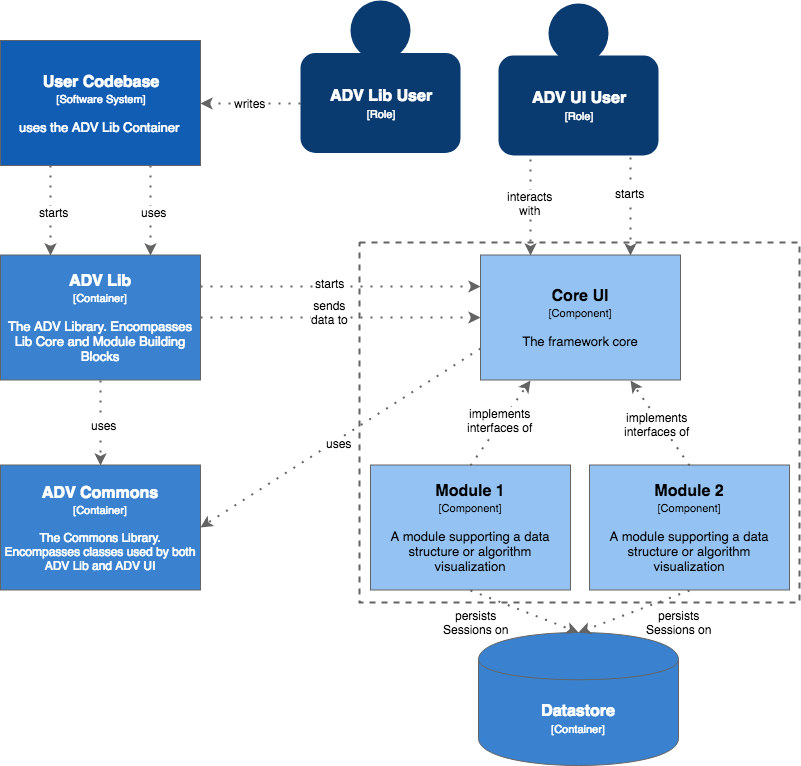
\includegraphics[width=0.7\textwidth]{attachments/c4/component-ui-diagram}
	\caption{Offizielle C4 Übersicht~\cite{c4}}
	\label{fig:c4-overview}
\end{figure}


\subsection{Code Listing}
\begin{lstlisting}[caption={Gradle}]
dependencies {
	compile 'ch.hsr.test:test:1.0'
}
\end{lstlisting}

Inline Code: \lstinline|java -jar test-<version>.jar|

\subsection{Image Explanation}
\begin{explanation}{attachments/c4/component-ui-diagram}
	Image Explanation
\end{explanation}

Circles with numbers to reference images: Click on button \circled{1}, \circled{2}, \circled{3a}


\subsection{Dir Tree}
\begin{table}[H]
	\centering
	\begin{tabularx}{\linewidth}{X X}
		\toprule 
		Projekt A & Projekt B \\
		\midrule
		\dirtree{%
			.1 A.
			.2 A1.
			.2 A2.
			.2 A3.
			.2 A4.
			.3 src.
			.4 main.
			.5 java.
			.6 C.
		}
		& 
		\dirtree{%
			.1 A.
			.2 A1.
			.2 A2.
			.2 A3.
			.2 A4.
			.3 src.
			.4 main.
			.5 java.
			.6 C.
		}
		\\
		\bottomrule 
	\end{tabularx} 
	\caption{Projekt Struktur} 
	\label{tbl:project-structure}
\end{table}


\subsection{Hints and Warnings}
\begin{hint}{Hint}{}
	See theoremsetup.tex
\end{hint}

\begin{warn}{Warning}{}
	See theoremsetup.tex
\end{warn}


\chapter{Projektplanung}
\begin{table}[H]
	\centering
	\begin{tabularx}{\linewidth}{l l X l}
		\toprule 
		Datum & Version & Änderungen & Autor \\
		\midrule
		DATE & VERSION & DESCRIPTION & AUTHOR \\
		\bottomrule 
	\end{tabularx} 
	\caption{Versionshistory Projektplanung} 
\end{table}

\section{Zeitplanung} 

\section{Projektverwaltung} 


\subsection{Iterationsplanung} \label{phasen}

\subsection{Schätzungen}

\subsection{Zeitauswertung}

\section{Meilensteine} \label{milestones}

\subsection{Artefakt Übersicht}

\section{Meetings} \label{meeting} 

\section{Verantwortlichkeiten}

\section{Repositories} \label{repositories}

\section{Entwicklungs Konzept}

\subsection{Definition of Done} \label{dod} 

\subsection{Buildprozess} \label{buildprocess}

\subsection{Continuous Integration}

\subsection{Review} \label{review}

\section{Backups} \label{backup}

\section{Risikomanagement} \label{tbl:risktable}

\begin{landscape}
	\LTXtable{\linewidth}{tables/table-risklist.tex}
\end{landscape}

\section{Qualitätsattribute} \label{quality-attributes}

\section{Exception Handling}

\section{Logging} \label{logging}

\section{Testing}

% Appendix
% ====================
\part{Anhang}
\appendix

\chapter{Aufgabenstellung} \label{appendix:aufgabenstellung}



\chapter{Klassendiagramme} \label{appendix:class-diagrams}

% \includepdf[pages=-]{attachments/a/b}

% \includepdf[pages=-,fitpaper]{attachments/a/b}

% \includepdf[pages=-, landscape=true]{attachments/a/b}

\chapter{Sequenzdiagramme} \label{appendix:sequence-diagrams}


\chapter{Testprotokolle} \label{appendix:test-protocols}

\section{Systemtests} \label{appendix:system}

\section{Usability Tests} \label{appendix:usability}


\chapter{Metriken} \label{appendix:metrics}


\chapter{Benutzerhandbuch}

\section{Installationsanleitung}

\chapter{Persönliche Berichte}

\section{Author A}


\section{Author B}


\chapter{Zeitauswertung} \label{appendix:zeitauswertung}

\section{Zeitauswertung nach Kategorien}

\section{Zeitauswertung nach Meilensteinen}

\section{Zeitauswertung nach Teammitgliedern}

\section{Zeitauswertung Soll-Ist-Vergleich}


\chapter{Meeting Protokolle}
\label{minutes}
\section{Meeting Protokoll Woche 1}

\begin{table}[h!]
	\begin{tabularx}{\textwidth}{l X }

		Ort & UPDATE ROOM \\
		Datum & UPDATE DATE \\
		Uhrzeit & UPDATE TIME \\
		Teilnehmer & 
		\begin{minipage}[t]{\textwidth}
			\begin{itemize}
				\item PARTICIPANT 1
				\item PARTICIPANT 2
				\item PARTICIPANT 3
			\end{itemize}
		\end{minipage}
	\end{tabularx}
\end{table}

\paragraph{Rückblick}
\begin{enumerate}
	\item A
\end{enumerate}

\paragraph{Aktuelles}
\begin{enumerate}
	\item B
\end{enumerate}

\paragraph{Beschlüsse}
\begin{enumerate}
	\item C
\end{enumerate}

\paragraph{Ausblick}
\begin{enumerate}
	\item D
\end{enumerate}


\paragraph{Nächster Termin} \hfill
\begin{table}[h!]
	\begin{tabularx}{\textwidth}{l X }
		Termin & 01.03.2018 \\
		Bemerkungen & - \\
	\end{tabularx}
\end{table}

\clearpage

\backmatter

% Bibliography
% ====================
\cleardoublepage
\printbibliography[title={Literaturverzeichnis}]

% Declarations
% ====================
\chapter{Vereinbarung über Urheber- und Nutzungsrechte}



\end{document}
